\documentclass[11pt,a4paper]{article}
\usepackage{fontspec}
\setmainfont{TeX Gyre Pagella}
\newfontfamily\headfont{Inter}[UprightFont=*-ExtraBold,BoldFont=*-ExtraBold,Extension=.otf,Path=/usr/share/fonts/opentype/inter/]
\usepackage[a4paper,margin=2.3cm]{geometry}
\usepackage{graphicx,booktabs,float,caption,array,xcolor,longtable}
\usepackage{xurl}
\usepackage[hidelinks]{hyperref}
\usepackage{titlesec}
\usepackage[round]{natbib}
\usepackage{setspace}
\setstretch{1.05}
\renewcommand{\topfraction}{0.9}
\renewcommand{\bottomfraction}{0.8}
\renewcommand{\textfraction}{0.1}
\renewcommand{\floatpagefraction}{0.75}
\setlength{\parindent}{0pt}
\setlength{\parskip}{0.55em}
\titleformat{\section}{\headfont\Large}{\thesection}{0.8em}{}
\titleformat{\subsection}{\headfont\large}{\thesubsection}{0.8em}{}
\captionsetup{font=small,labelfont=bf}
\urlstyle{same}
\hypersetup{pdftitle={The Largest City on Earth},pdfauthor={Tristan Hotham}}

\begin{document}
\begin{center}
{\Large\bfseries The Largest City on Earth\par}
\vspace{0.4em}
{\large Six thousand years of the world's biggest cities, 3700 BC to AD 2050:\\Chandler, Modelski and the UN World Urbanization Prospects 2025\par}
\vspace{1.2em}
{\large Tristan Hotham\par}
\vspace{0.3em}
{\small Independent researcher\\
ORCID: 0000-0003-4931-9349\\
DOI: https://doi.org/10.5281/zenodo.23872999\par}
\vspace{0.8em}
2026
\end{center}

\begin{quote}
\small
\begin{center}\textbf{Abstract}\end{center}
I trace the largest city in the world from 3700 BC to the United Nations' projections for 2050, combining Reba, Reitsma and Seto's (2016) geocoded versions of Chandler's (1987) and Modelski's (2003) compilations (1,654 places and 10,033 population estimates after cleaning) with the UN World Urbanization Prospects 2025, which defines cities by the Degree of Urbanisation. At 85 snapshot dates, 30 different cities are the largest on their own. Uruk leads from 3500 to 2800 BC with up to 80,000 people; the crown then passes among Sumerian, Egyptian and Mesopotamian cities, to Linzi, Alexandria and Rome, to Constantinople, Chang'an and Baghdad, and for most of 1100 to 1825 to Chinese capitals (Chinese in 13 of 16 snapshots). London leads from 1850 to 1914, roughly 1826 to 1925 by interpolation; New York, Tokyo and, in the UN's figures, Jakarta (41.9 million in 2025) follow, and Dhaka is projected to pass Jakarta in 2049 by a margin of 0.7\%. The largest city first reaches 100,000 in 2100 BC and a million in 100 BC in Modelski's figures, but in the combined estimates never exceeds 900,000 between 1100 and 1750. The population-weighted centre of the 25 largest places stays near Mesopotamia until about 800 BC, sits over Central Asia from AD 500 to 1825, swings to the North Atlantic between 1850 and 1970, and returns to Asia, reaching 31°N 95°E in 2025. The two historical compilations name different leaders at 10 of 15 comparable snapshots, and the 1975 seam between historical and DEGURBA figures changes rankings substantially; both are documented rather than smoothed.

\textbf{Keywords:} cities; urbanisation; historical demography; urban history; Chandler; Modelski; World Urbanization Prospects; Degree of Urbanisation; open data; mapping
\end{quote}

\section{Introduction}
Lists of the largest city in history are popular and unstable. They depend on whose estimates are used, on what counts as a city, and on how sparse records from different centuries are put side by side. This paper builds such a list transparently from open data. It asks four questions: which city was the largest at each moment from 3700 BC to the UN's projections for 2050, how large it was, how the geographic centre of the world's big cities moved, and how much the answers depend on the sources and definitions. It accompanies an interactive map (\url{https://maps.tristanhotham.com/largest-cities/}).

\section{Data}
\textbf{Historical compilations.} \citet{reba} digitised and geocoded two compilations: Tertius Chandler's \textit{Four Thousand Years of Urban Growth} \citep{chandler} and George Modelski's \textit{World Cities} \citep{modelski}. Their files on figshare \citep{figc,figa,figm} are wide tables of places (name, other names, country, coordinates, a certainty score from 1 to 3) with population figures by date. Chandler's file has 1,597 places and 9,438 figures between 2250 BC and 1975, at 798 distinct dates; Modelski's ancient file has 154 places and 621 figures on a grid of 41 dates from 3700 BC to AD 1000, listing places of 10,000 or more before 1000 BC and of 100,000 or more after; his modern file lists 293 cities of a million or more in AD 2000. I used the V2 files. Compared with V1 they trim leading and trailing spaces from 73 names and countries (3 remain), correct ``Instanbul'' to Istanbul, assign Kiev to Ukraine rather than the Russian Federation, and merge V1's duplicate Guadalajara row and a misspelt ``Madgdeburg'' row into one row each, so that Chandler has 1,597 rows rather than 1,599; no population figure differs. The files are Windows-1252 text; read as UTF-8 they fail, and read as Latin-1 they corrupt names such as Košice. 3 alternative names had already lost characters, stored as question marks.

\textbf{UN World Urbanization Prospects 2025.} Files 18 to 21 of the 2025 revision \citep{wup} give the 100 largest cities at each five-year date, the 100 largest of 2025 through time, capital cities, and the population of all 16,828 cities that reach 50,000 between 1975 and 2050, annually, with population-weighted centroids and a plausibility rating. Cities are defined by the Degree of Urbanisation: contiguous 1 km\textsuperscript{2} grid cells with at least 1,500 inhabitants per km\textsuperscript{2} and at least 50,000 inhabitants in all. I checked that file 18's rankings and file 19's 2025 list agree exactly with file 21. Country outlines are from Natural Earth \citep{ne}.

\section{Methods}
\subsection{Corrections}
I made 26 documented corrections (Table~\ref{tab:fixes}). The main one is systematic: every BC figure for Modelski's cities in the Americas is an exact copy of the AD figure 1,300 years later (for example Teotihuacan at 100,000, 150,000, 100,000 and 100,000 in 900 to 600 BC and in AD 400 to 700), so I dropped the 14 copies. I dropped single figures out by about a factor of ten from the same place's neighbouring figures, figures attached to the wrong place, and 2 zero values, and moved two misplaced locations. Rows with the same name less than 5 km apart were merged.

\begin{longtable}{lllrp{6.2cm}}\caption{Corrections to the V2 files.}\label{tab:fixes}\\\toprule Source & Place & Date & Figure & Reason\\\midrule\endfirsthead\toprule Source & Place & Date & Figure & Reason\\\midrule\endhead
Modelski & Caracol & 900 BC & 100,000 & copy of the AD figure 1,300 years later\\
Modelski & Caracol & 800 BC & 100,000 & copy of the AD figure 1,300 years later\\
Modelski & Caracol & 700 BC & 140,000 & copy of the AD figure 1,300 years later\\
Modelski & Caracol & 600 BC & 100,000 & copy of the AD figure 1,300 years later\\
Modelski & Caracol & 500 BC & 100,000 & copy of the AD figure 1,300 years later\\
Modelski & Teotihuacan & 900 BC & 100,000 & copy of the AD figure 1,300 years later\\
Modelski & Teotihuacan & 800 BC & 150,000 & copy of the AD figure 1,300 years later\\
Modelski & Teotihuacan & 700 BC & 100,000 & copy of the AD figure 1,300 years later\\
Modelski & Teotihuacan & 600 BC & 100,000 & copy of the AD figure 1,300 years later\\
Modelski & Tiahuanaco & 500 BC & 100,000 & copy of the AD figure 1,300 years later\\
Modelski & Tikal & 900 BC & 100,000 & copy of the AD figure 1,300 years later\\
Modelski & Tikal & 800 BC & 100,000 & copy of the AD figure 1,300 years later\\
Modelski & Tikal & 600 BC & 100,000 & copy of the AD figure 1,300 years later\\
Modelski & Tollan & 300 BC & 100,000 & copy of the AD figure 1,300 years later\\
Chandler & Philadelphia & AD 1914 & 17,600,000 & ten times the 1900 and 1925 figures (an extra digit)\\
Chandler & Algiers & AD 1925 & 2,220,000 & sixteen times 1900 and five times 1950 (an extra digit)\\
Chandler & Nanjing & AD 1970 & 200,000 & a fifth of 1950 and a tenth of 1975 (a missing digit)\\
Chandler & Palermo & AD 1150 & 125 & 125 people between 90,000 and 150,000\\
Chandler & Delhi & AD 1375 & 1,250,000 & ten times the 1354 and 1398 figures (an extra digit)\\
Chandler & Memphis & AD 1975 & 846,000 & the figure for Memphis, Tennessee\\
Chandler & Gelibolu & AD 1000 & 300,000 & repeats Constantinople's figure\\
Chandler & Gelibolu & AD 1200 & 150,000 & repeats Constantinople's figure\\
Chandler & London & 100 BC & 30,000 & before the Roman foundation of London\\
Modelski 2000 & Montevideo & AD 2000 & 13,303,000 & ten times the city's population (an extra digit)\\
Modelski & Shangqi &  & location & geocoded on Shanghai; moved to Shangqiu, Henan\\
Modelski & Caracol &  & location & geocoded on El Caracol, Chichen Itza; moved to Caracol, Belize\\
\bottomrule\end{longtable}

\subsection{Places and snapshots}
I matched 95 places across the two compilations by name or alternative name and distance (under 30 km), giving 1,654 places. Snapshots are Modelski's dates to AD 1000 plus Chandler's cross-sections in 1360, 650 and 430 BC and AD 361 and 622, then Chandler's benchmark years from 1100 to 1970, then the UN every five years from 1975 to 2050: 85 in all. At each snapshot each compilation gives a place its own figure for that date if it has one. Otherwise Chandler's figure is interpolated log-linearly between his two nearest dates for the place if they are at most 300 years apart (before AD 1000), 200 years (to 1800) or 100 years (after); Modelski's figures are interpolated only between adjacent dates of his grid. Nothing is extrapolated. The combined estimate is the mean of the compilations that give one. Places within 0.5\% of the top are treated as tied. From 1975 only the UN figures are used; the two definitions are not blended.

\subsection{Centre of gravity, counts and links}
The centre of gravity at each snapshot is the population-weighted mean of the unit vectors of the 25 largest places (and, as a check, the 10 largest), projected back to the sphere. Counts of places of 100,000 and of a million or more are counts within the compilations before 1975 and are therefore lower bounds. I linked 1,129 historical places to the UN city containing them (same name within 50 km), which allows a place's history to run across the seam.

\section{Results}
\subsection{The succession}
Figure~\ref{fig:crown} and Table~\ref{tab:reigns} give the succession. Modelski's first date, 3700 BC, lists only Eridu (6,000). Uruk leads from 3500 to 2800 BC, reaching 80,000, and is not beaten until Ur in 2100 BC. Lagash, Mari and Girsu follow; Ur is the first place of 100,000 in 2100 BC. In 2000 BC Chandler's Memphis (60,000) leads because the compilations disagree on Ur (65,000 in Chandler, 20,000 in Modelski). Egyptian capitals lead in 7 of the 8 snapshots between 1600 and 1000 BC; Yin leads in 1300 BC. From 1000 BC Modelski's threshold of 100,000 produces ties (Babylon, Memphis and Thebes in 900 and 800 BC; 5 places in 700 BC). Linzi leads in 500 and 300 BC, Alexandria in 200 and 100 BC (Modelski's 1,000,000 in 100 BC is the first million), and Rome from AD 1 to 400. Constantinople (500 and 600), Ctesiphon (622), Chang'an (700), Baghdad (tied with Chang'an in 800; alone in 900 and 1000), Kaifeng (1100), Merv (1150), Hangzhou (1200 to 1350), Nanjing (1400) and Beijing (1450 to 1600; 1750 to 1825) follow, with Istanbul in 1650 and 1700. London leads from 1850 to 1914, ties with New York in 1925, and New York leads in 1950. Tokyo leads from Chandler's 1970 figure through the UN's 1975 to 2005; Jakarta ties with Tokyo in 2010 and leads from 2015 to 2045; Dhaka leads in 2050.

\begin{figure}[tbp]\centering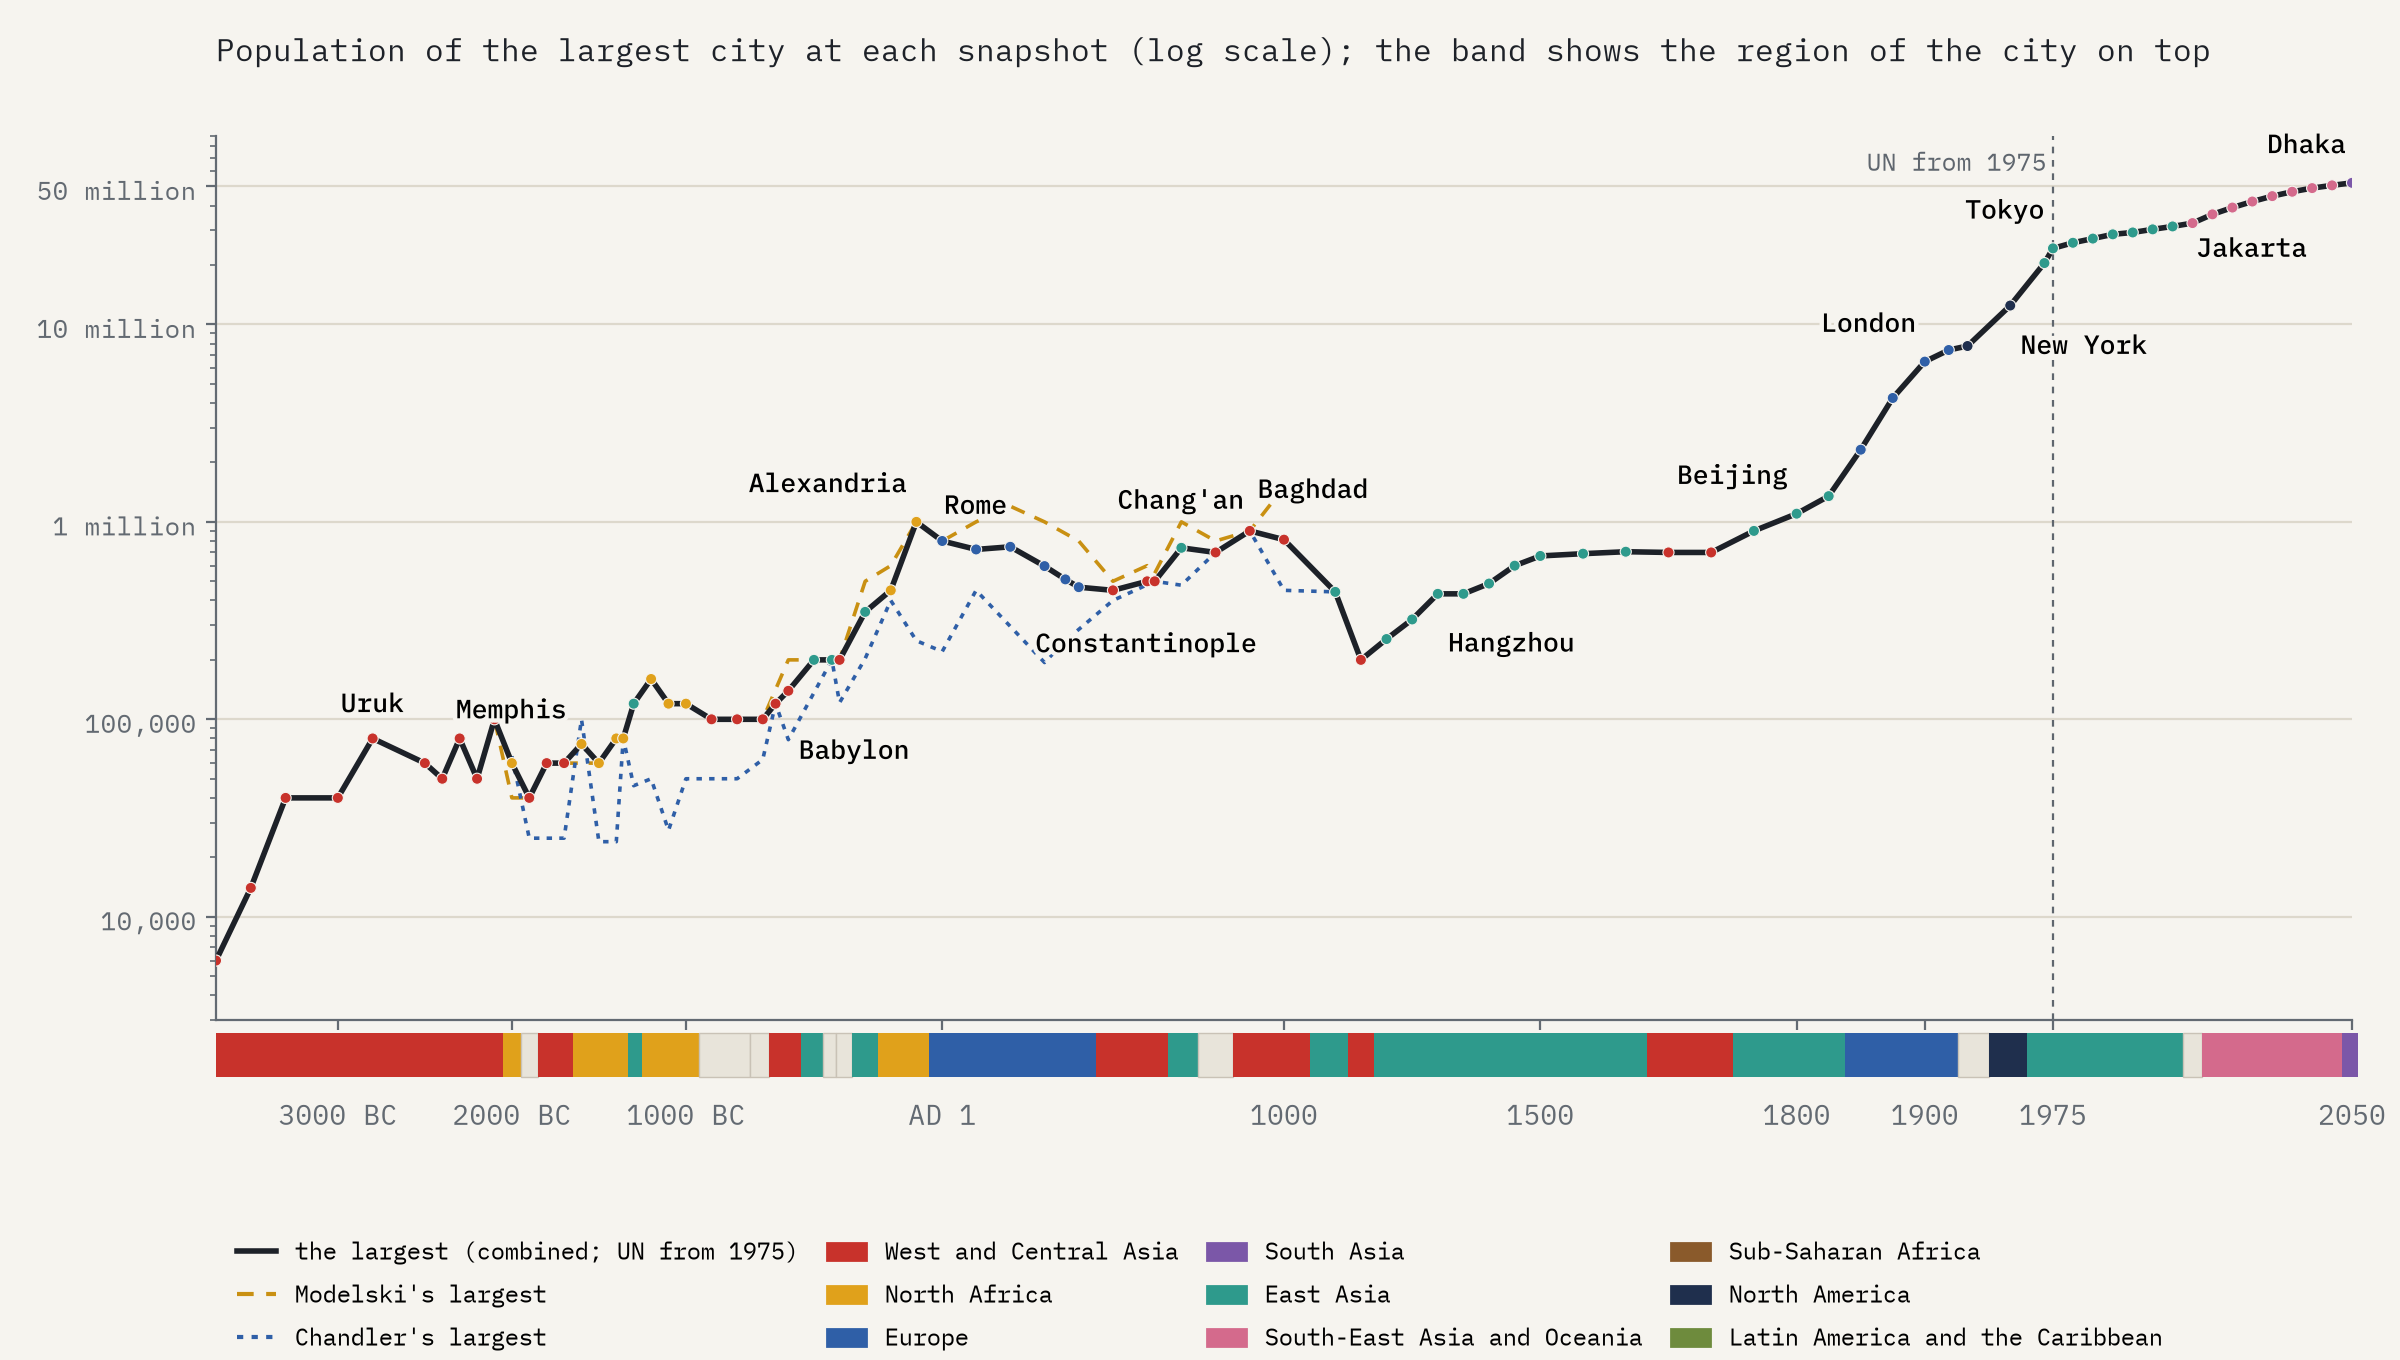
\includegraphics[width=\textwidth]{f_crown.png}
\caption{Population of the largest place at each snapshot (log scale), the largest in each compilation alone (dashed), and the region of the leader (band). The UN figures begin in 1975.}\label{fig:crown}\end{figure}

\begin{longtable}{llp{6.6cm}rr}\caption{Every run of consecutive snapshots with the same largest place (ties listed separately), with the highest population in the run.}\label{tab:reigns}\\\toprule From & To & Largest place & Snapshots & Peak\\\midrule\endfirsthead\toprule From & To & Largest place & Snapshots & Peak\\\midrule\endhead
3700 BC &  & Eridu & 1 & 6,000\\
3500 BC & 2800 BC & Uruk & 4 & 80,000\\
2500 BC &  & Lagash & 1 & 60,000\\
2400 BC &  & Mari & 1 & 50,000\\
2300 BC & 2200 BC & Girsu & 2 & 80,000\\
2100 BC &  & Ur & 1 & 100,000\\
2000 BC &  & Memphis & 1 & 60,000\\
1900 BC &  & Isin and Larsa (tie) & 1 & 40,000\\
1800 BC &  & Mari & 1 & 60,000\\
1700 BC &  & Babylon & 1 & 60,000\\
1600 BC &  & Avaris & 1 & 75,000\\
1500 BC & 1360 BC & Thebes & 3 & 80,000\\
1300 BC &  & Yin & 1 & 120,000\\
1200 BC & 1100 BC & Pi-Ramesses & 2 & 160,000\\
1000 BC &  & Thebes & 1 & 120,000\\
900 BC & 800 BC & Babylon, Memphis and Thebes (tie) & 2 & 100,000\\
700 BC &  & Babylon, Linzi, Memphis, Nineveh and Thebes (tie) & 1 & 100,000\\
650 BC &  & Nineveh & 1 & 120,000\\
600 BC &  & Babylon & 1 & 139,442\\
500 BC &  & Linzi & 1 & 200,000\\
430 BC &  & Babylon and Linzi (tie) & 1 & 200,000\\
400 BC &  & Babylon, Kaifeng and Linzi (tie) & 1 & 200,000\\
300 BC &  & Linzi & 1 & 350,000\\
200 BC & 100 BC & Alexandria & 2 & 1.00m\\
AD 1 & AD 400 & Rome & 6 & 800,000\\
AD 500 & AD 600 & Constantinople & 2 & 500,000\\
AD 622 &  & Ctesiphon & 1 & 500,000\\
AD 700 &  & Chang'an & 1 & 738,888\\
AD 800 &  & Baghdad and Chang'an (tie) & 1 & 700,000\\
AD 900 & AD 1000 & Baghdad & 2 & 900,000\\
AD 1100 &  & Kaifeng & 1 & 442,000\\
AD 1150 &  & Merv & 1 & 200,000\\
AD 1200 & AD 1350 & Hangzhou & 4 & 432,000\\
AD 1400 &  & Nanjing & 1 & 487,000\\
AD 1450 & AD 1600 & Beijing & 4 & 706,000\\
AD 1650 & AD 1700 & Istanbul & 2 & 700,000\\
AD 1750 & AD 1825 & Beijing & 3 & 1.35m\\
AD 1850 & AD 1914 & London & 4 & 7.42m\\
AD 1925 &  & London and New York (tie) & 1 & 7.77m\\
AD 1950 &  & New York & 1 & 12.46m\\
AD 1970 & AD 2005 & Tokyo & 8 & 31.35m\\
AD 2010 &  & Jakarta and Tokyo (tie) & 1 & 32.60m\\
AD 2015 & AD 2045 & Jakarta & 7 & 50.61m\\
AD 2050 &  & Dhaka & 1 & 52.12m\\
\bottomrule\end{longtable}

\begin{figure}[tbp]\centering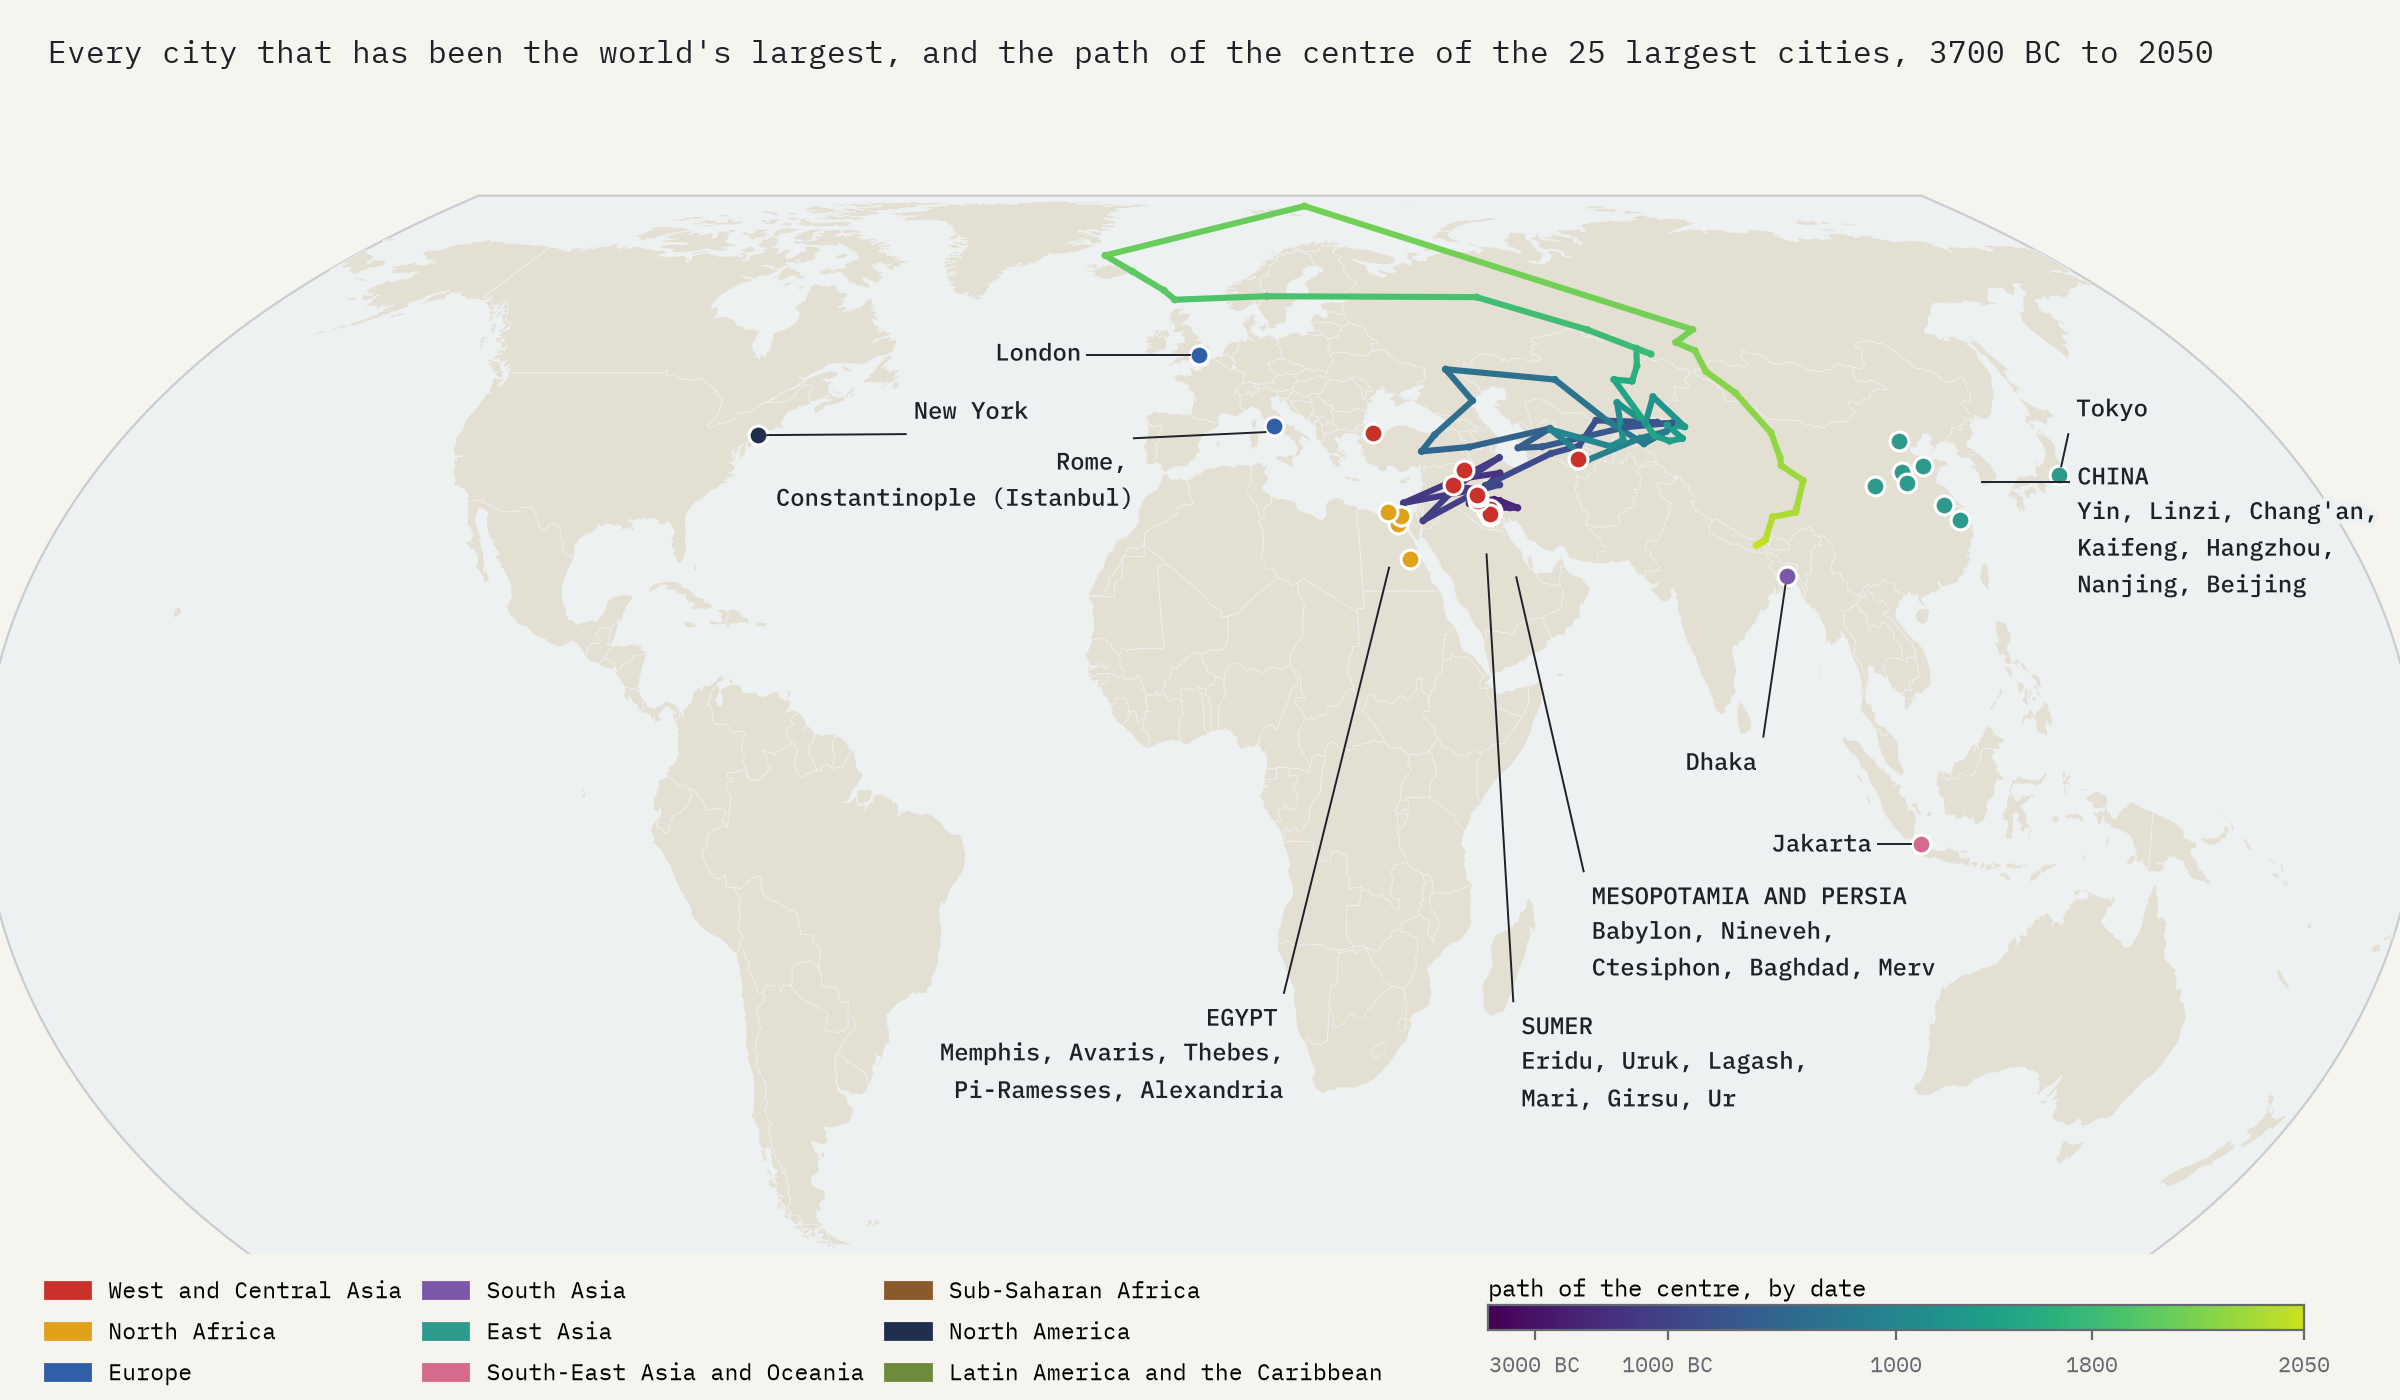
\includegraphics[width=\textwidth]{f_map.png}
\caption{Every place that has been the largest on its own, coloured by region, and the path of the population-weighted centre of the 25 largest places, coloured by date.}\label{fig:map}\end{figure}

\subsection{Size}
The largest place first passes a million in 100 BC in Modelski's figures; in Chandler's, at the snapshot dates, not until Beijing in 1800 (1,100,000), although his single figure for Baghdad in AD 932 is 1,100,000. Between 1100 and 1750 the combined estimate for the largest place never exceeds 900,000. London reaches 6,480,000 in 1900, New York 12,463,000 in 1950 and Tokyo 20,450,000 in Chandler's 1970 figure. The UN gives Tokyo 24,281,618 in 1975 and Jakarta 41,913,860 in 2025, and projects Dhaka at 52,122,843 in 2050. The compilations hold 51 places of 100,000 or more and 1 of a million in 1800, and 16 million cities in 1900; the UN counts 165 in 1975, 511 in 2025 and 611 in 2050 (Figure~\ref{fig:counts}).

\begin{figure}[tbp]\centering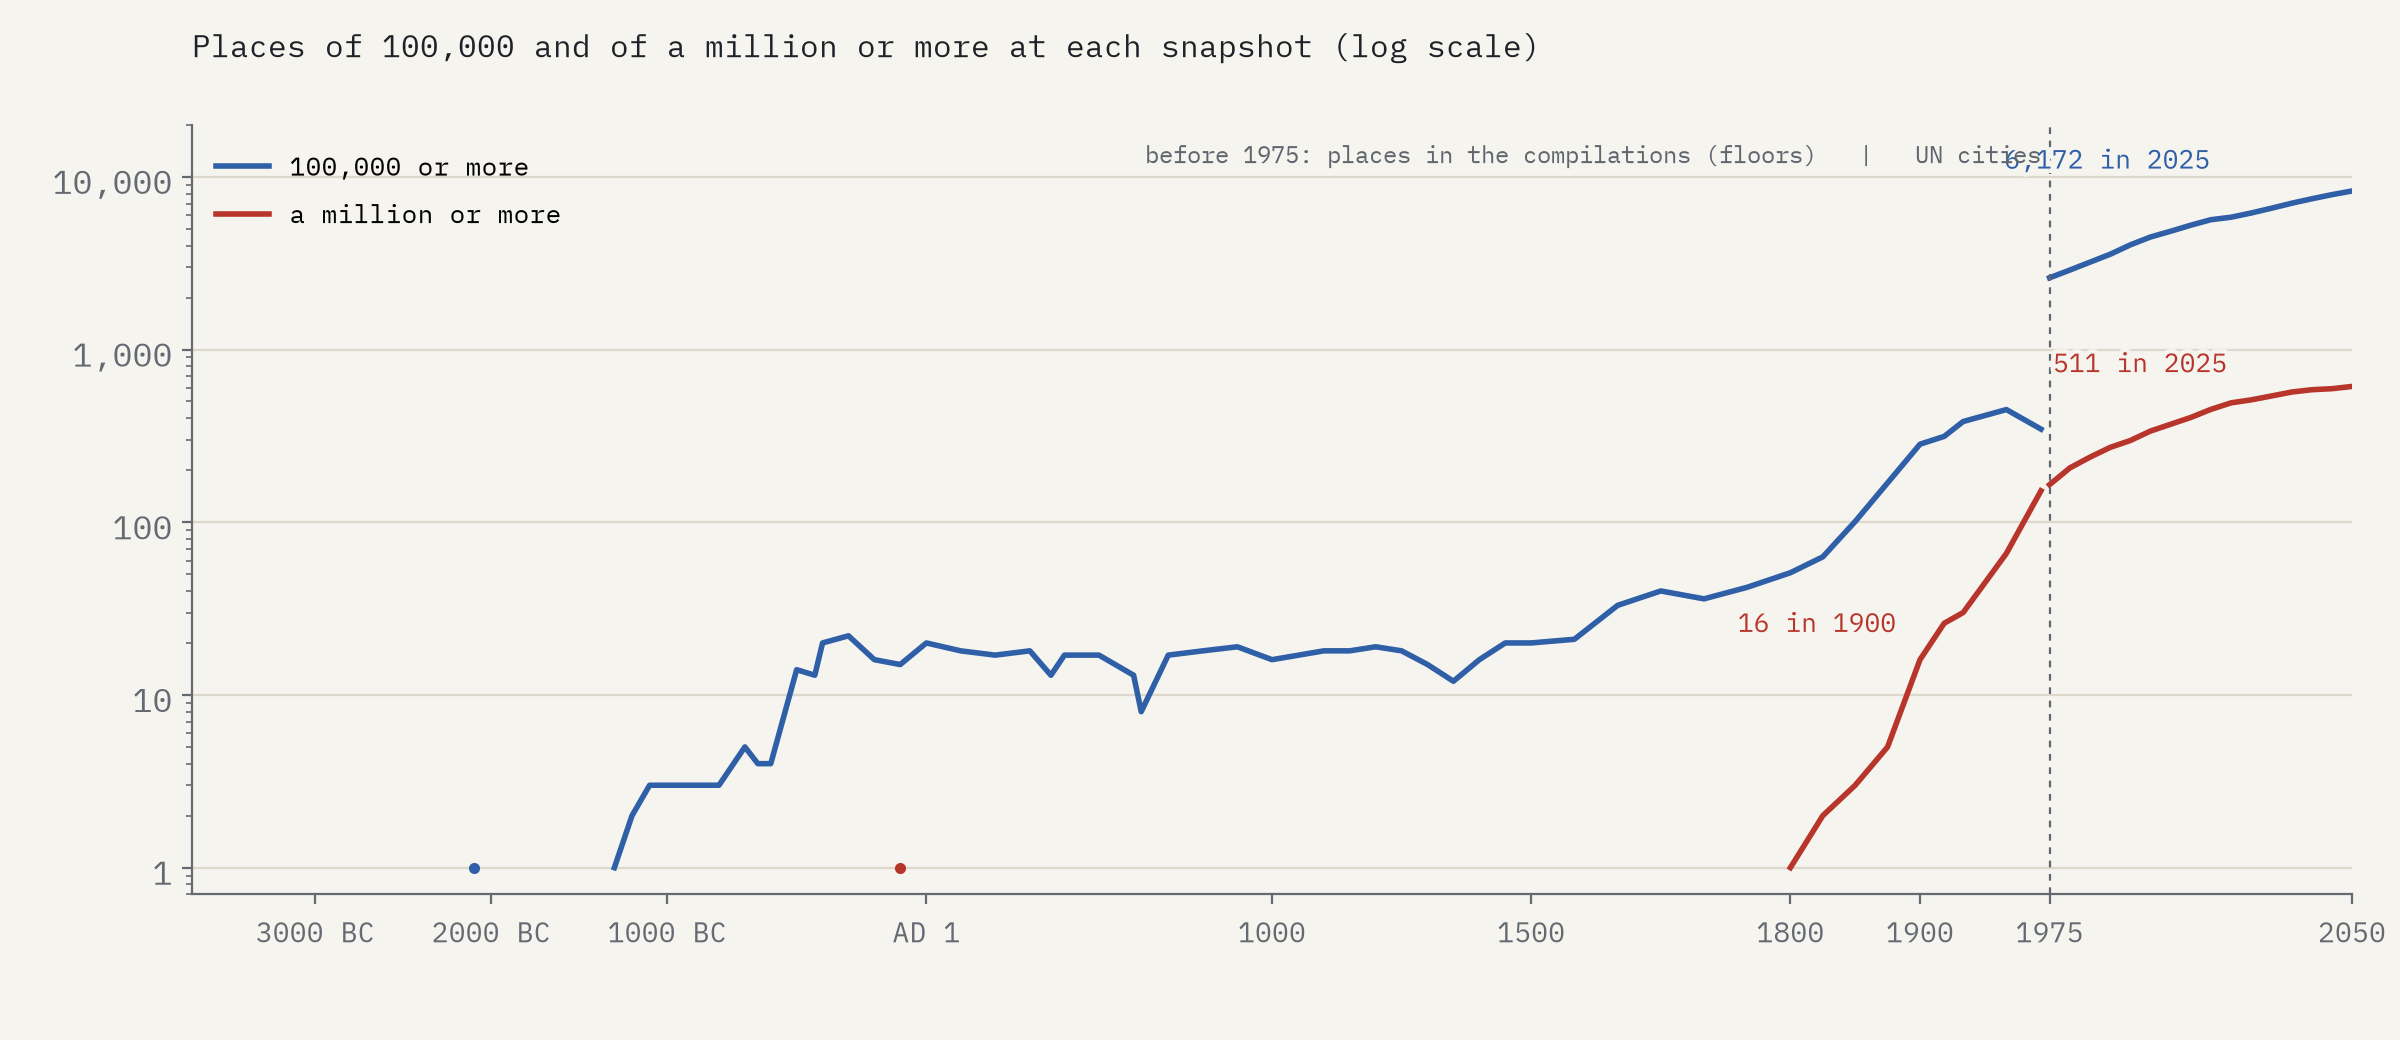
\includegraphics[width=\textwidth]{f_counts.png}
\caption{Places of 100,000 and of a million or more at each snapshot (log scale). Before 1975, counts within the compilations (lower bounds).}\label{fig:counts}\end{figure}

\subsection{Where the big cities were}
Figures~\ref{fig:regions} and \ref{fig:cog} show the regional make-up of the 25 largest places and the longitude of their centre. Until 800 BC the centre stays between 33°E and 51°E. It moves east to 77°E by 500 BC as Chinese and Indian cities enter the lists, back to 45°E in AD 100 under Rome's weight, and stays between 59°E and 82°E from AD 500 to 1825. In 1900 13 of the 25 largest places are European (59\% of their population) and the centre lies at 60°N 4.9°W, 5,102 km from its 1800 position; its westernmost point is in 1950 at 68°N. By 2025 it is at 31°N 95°E and by 2050 at 27°N 87°E; 19 of the 25 largest cities of 2025 are in Asia and 1 in Europe. A centre on the sphere is pulled poleward when the cities are spread around a hemisphere, which explains the high latitudes of the twentieth century; part of the jump at 1975 reflects the change of source.

\begin{figure}[tbp]\centering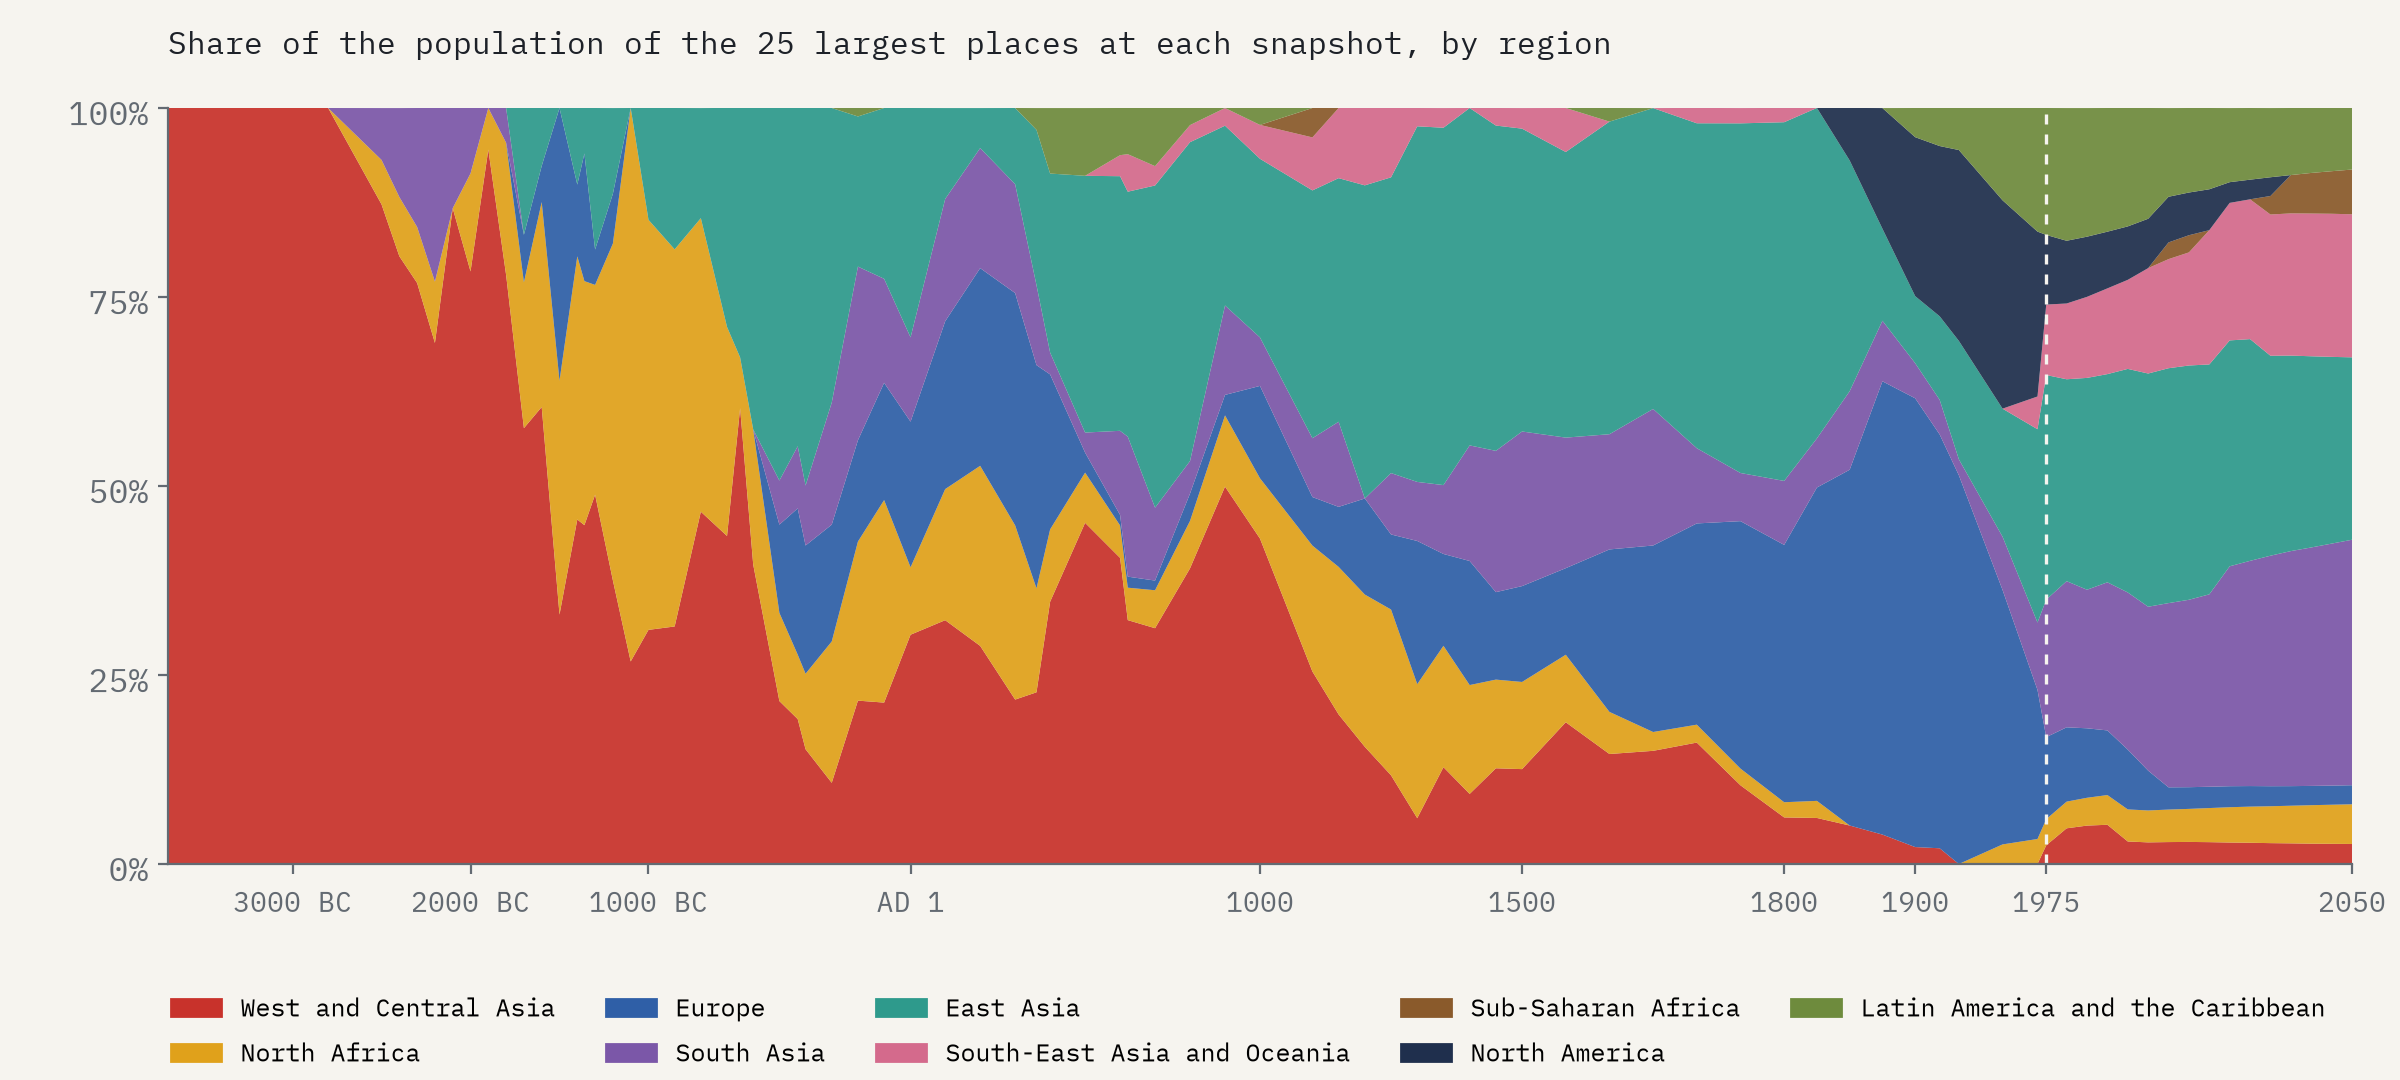
\includegraphics[width=\textwidth]{f_regions.png}
\caption{Share of the population of the 25 largest places by region at each snapshot.}\label{fig:regions}\end{figure}

\begin{figure}[tbp]\centering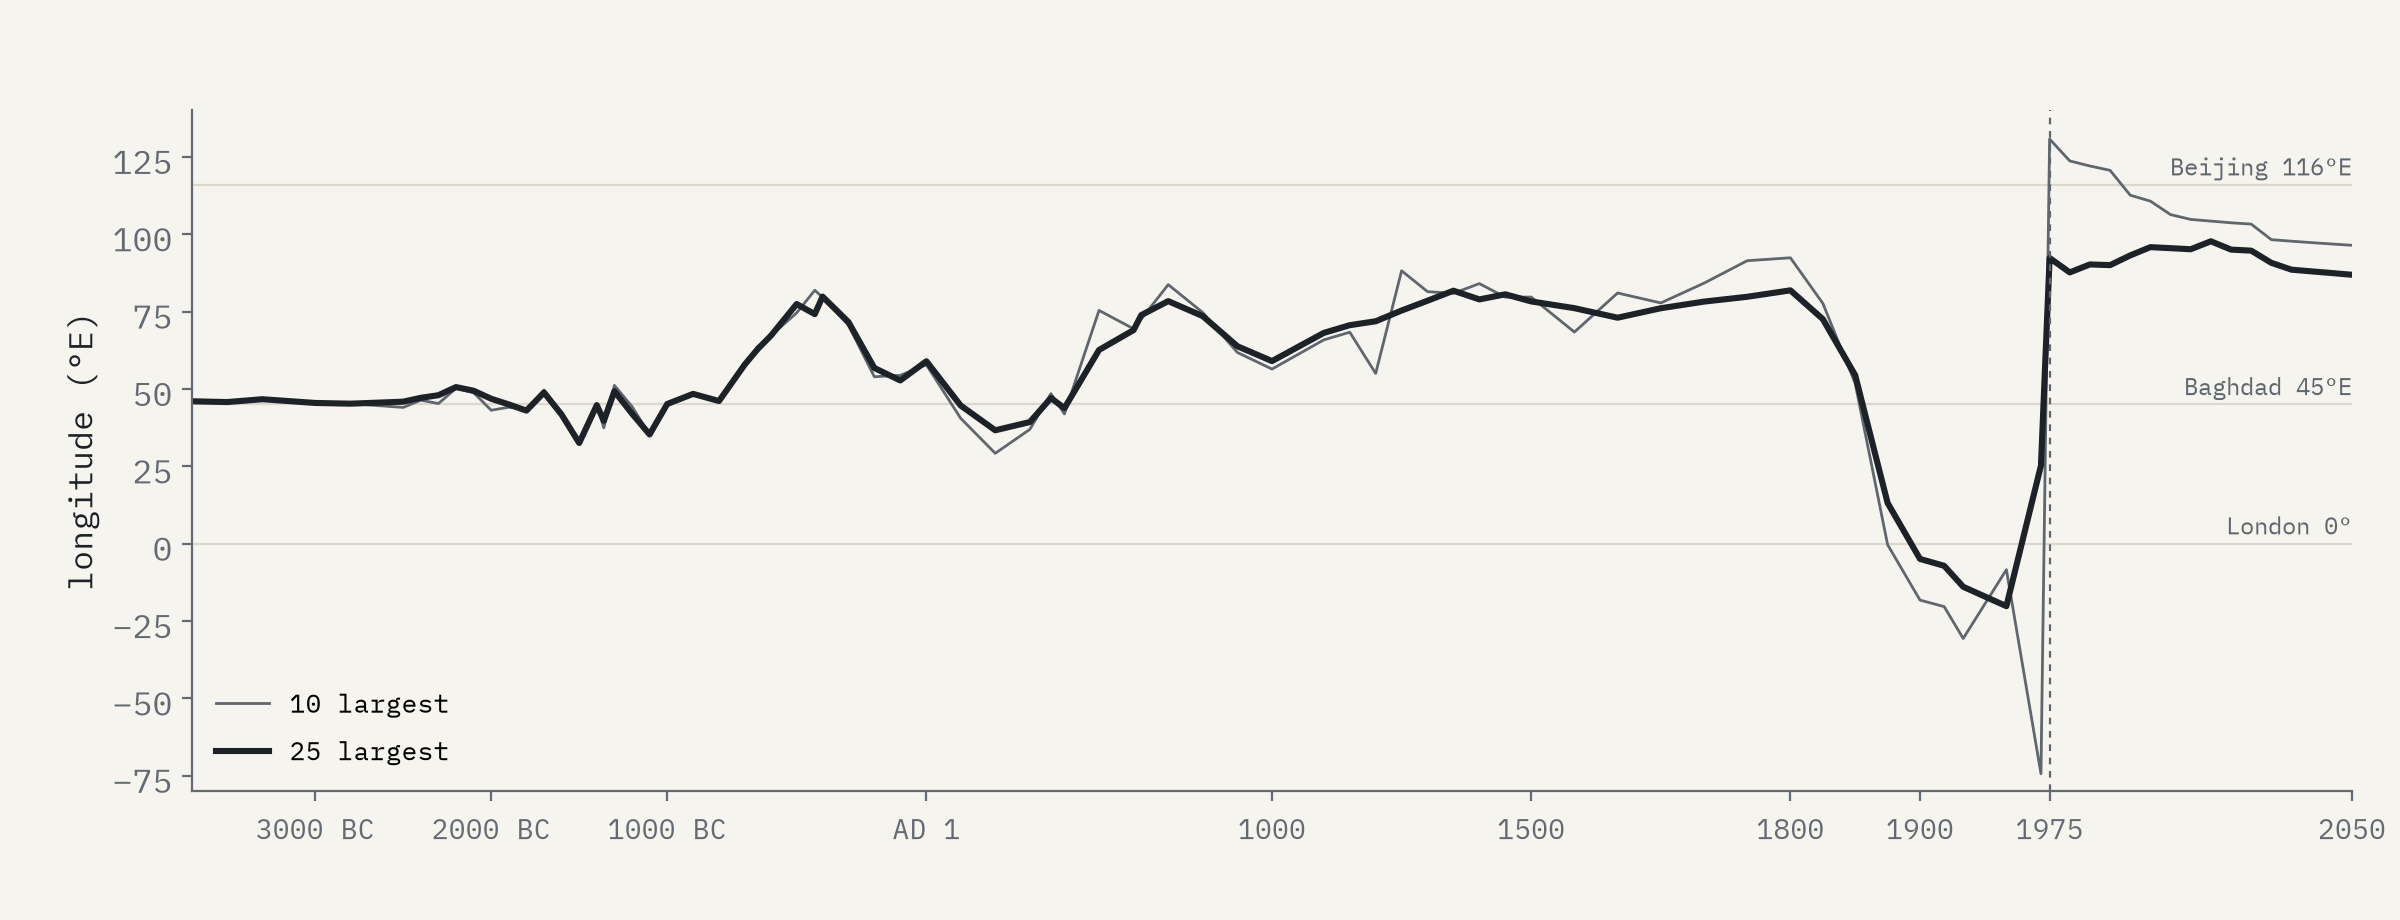
\includegraphics[width=\textwidth]{f_cog.png}
\caption{Longitude of the population-weighted centre of the 25 (thick) and 10 (thin) largest places.}\label{fig:cog}\end{figure}

\subsection{London}
London is 13th in 1600 (187,000), 4th in 1700, 3rd in 1750 and second to Beijing in 1800 (861,000 against 1,100,000). In 1825 it is 1.1\% behind Beijing; in 1850 it leads with 2,320,000, 1.41 times Beijing. In 1925 New York (7,774,000) and London (7,742,000) differ by 0.4\%. Linear interpolation between snapshots places London's lead at about 1826 to 1925 (99 years). Under the UN definition London has 10,416,420 people in 2025 and ranks 33rd (Figure~\ref{fig:london}).

\begin{figure}[tbp]\centering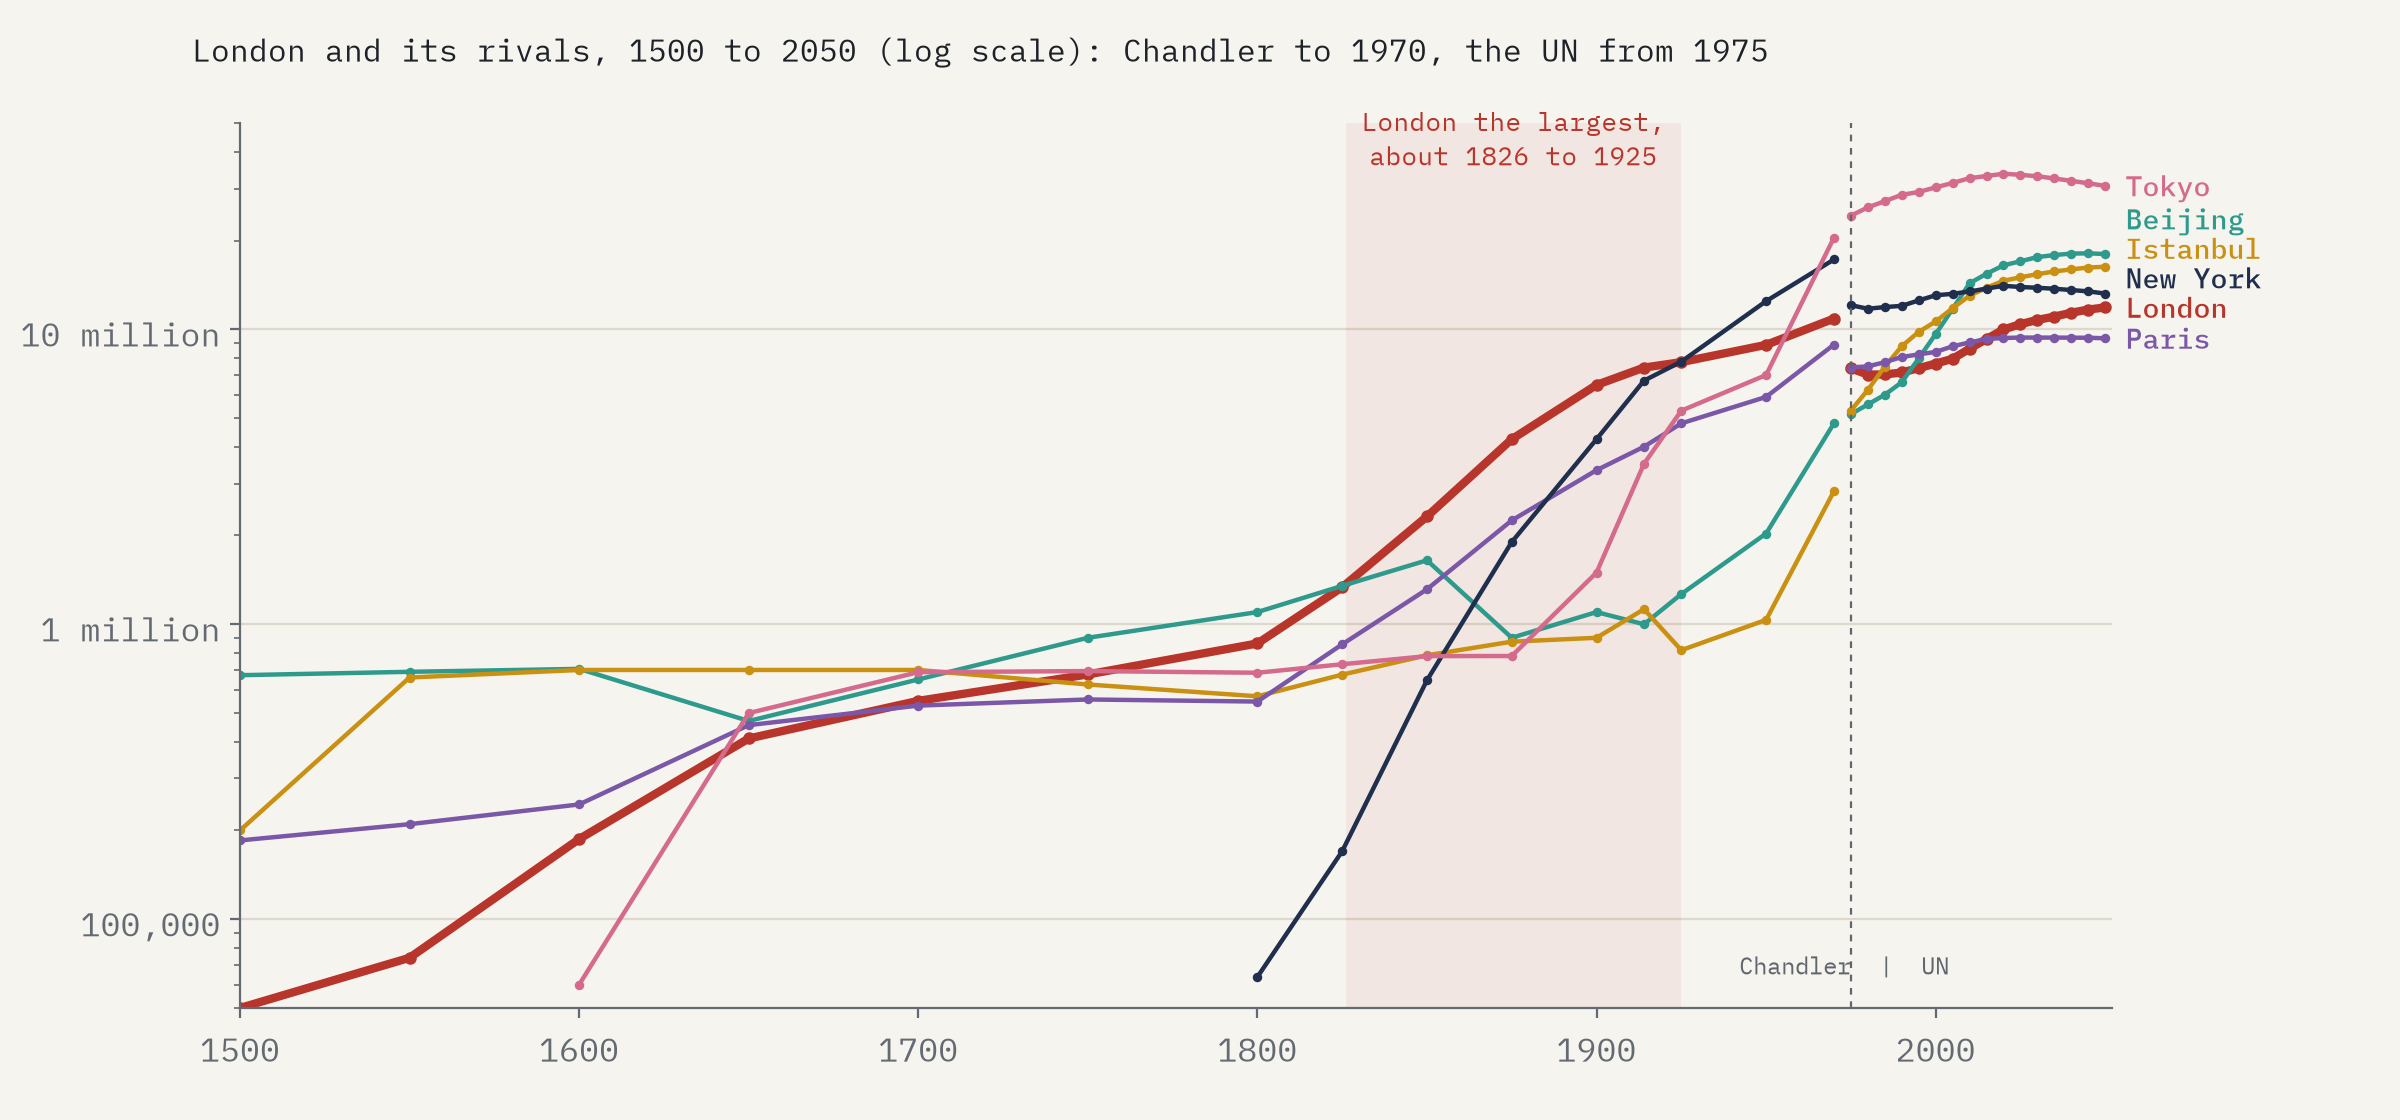
\includegraphics[width=\textwidth]{f_london.png}
\caption{London and its rivals, 1500 to 2050 (log scale): Chandler to 1970, the UN from 1975.}\label{fig:london}\end{figure}

\subsection{Agreement between the compilations}
At 15 snapshots both compilations have figures for at least 8 places; they name different leaders at 10 (Table~\ref{tab:dis}). In AD 1000 Modelski gives Baghdad 1,500,000 and Chandler 125,000, making Cordoba (450,000) his largest. Chandler's highest figures for ancient Rome and Alexandria are 38\% and 30\% of Modelski's. 73 of the 83 leaders before 1975 have certainty 1; the others are Hangzhou, Memphis and Pi-Ramesses.

\begin{table}[tbp]\centering\footnotesize\caption{Snapshots where both compilations have figures for at least 8 places and name different leaders.}\label{tab:dis}\begin{tabular}{lp{4.3cm}p{3.6cm}p{3.6cm}}\toprule Date & Modelski & Chandler & Combined\\\midrule
400 BC & Babylon, Kaifeng, Linzi, Luoyang, Carthage (200,000) & Syracuse (121,414) & Babylon, Kaifeng, Linzi\\
300 BC & Carthage (500,000) & Pataliputra (203,010) & Linzi\\
200 BC & Alexandria (600,000) & Chang'an (400,000) & Alexandria\\
100 BC & Alexandria (1.00m) & Seleucia (250,000) & Alexandria\\
AD 361 & Rome (872,740) & Ctesiphon (250,000) & Rome\\
AD 400 & Rome (800,000) & Ctesiphon (285,240) & Rome\\
AD 600 & Constantinople (600,000) & Ctesiphon (480,280) & Constantinople\\
AD 622 & Constantinople (548,796) & Ctesiphon (500,000) & Ctesiphon\\
AD 800 & Chang'an (800,000) & Baghdad (700,000) & Baghdad, Chang'an\\
AD 1000 & Baghdad (1.50m) & Cordoba (450,000) & Baghdad\\
\bottomrule\end{tabular}\end{table}

\subsection{The 1975 seam}
Chandler's 1975 list and the UN's 1975 figures describe the same year with different definitions (Figure~\ref{fig:seam}). Tokyo is similar (23,000,000 and 24,281,618); New York falls from 17,100,000 to 12,076,416 (3rd in the UN's ranking), and Jakarta rises from 5,300,000 (20th) to 11,696,369 (4th). Chandler lists 189 places of a million or more in 1975, the UN 165; Modelski lists 292 in 2000, the UN 337. DEGURBA also identifies very large ``cities'' in densely settled rural areas, such as Hajipur in Bihar (9,941,510 in 2025).

\begin{figure}[tbp]\centering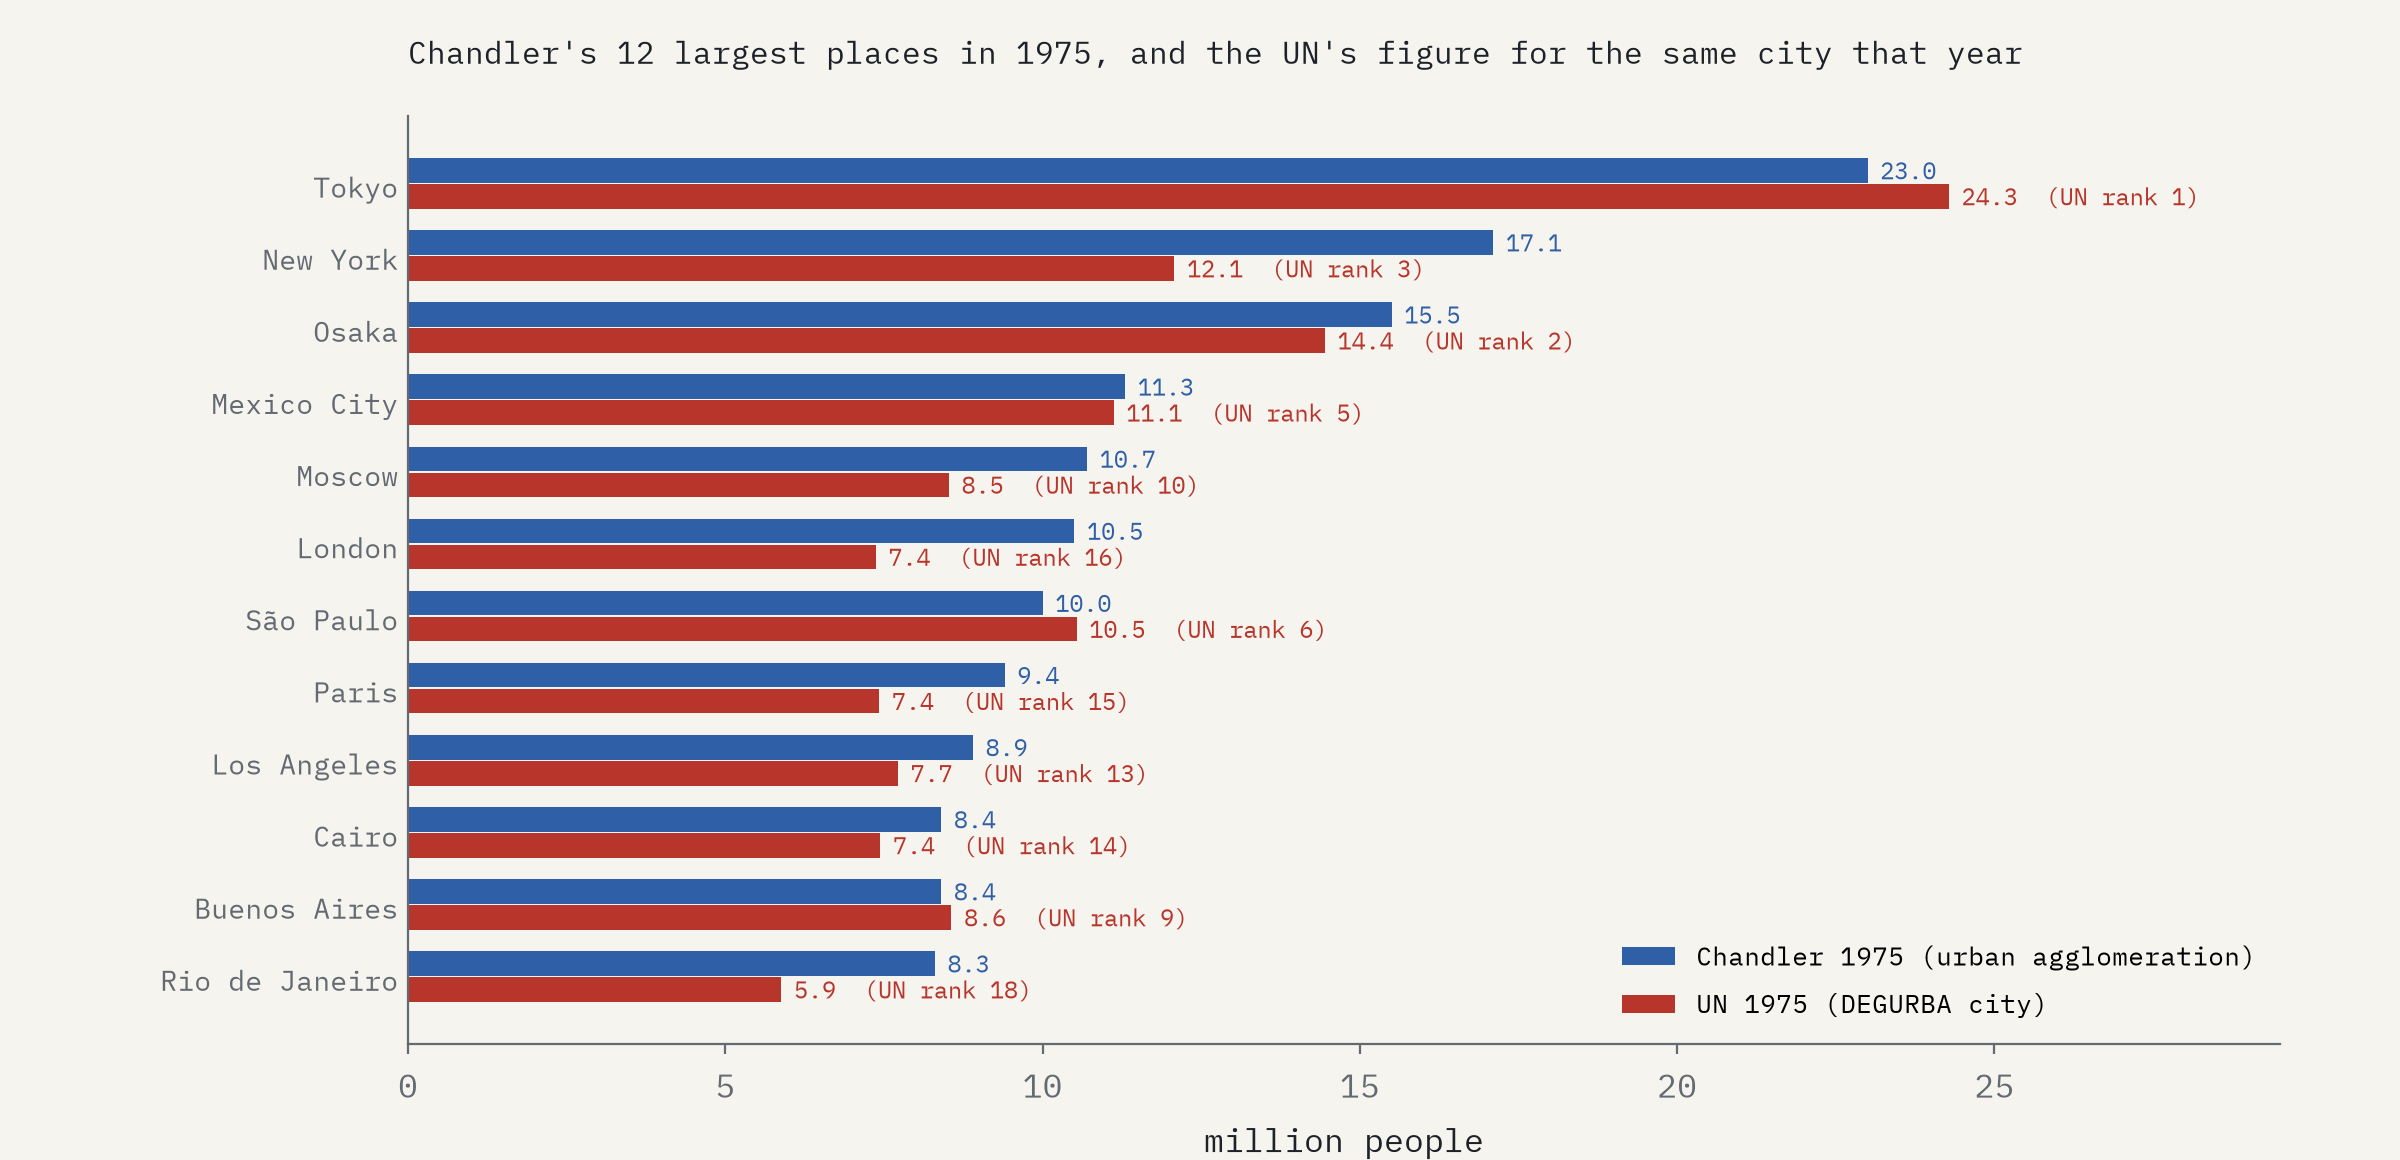
\includegraphics[width=\textwidth]{f_seam.png}
\caption{Chandler's 12 largest places in 1975 and the UN's figure for the city containing each.}\label{fig:seam}\end{figure}

\subsection{To 2050}
In the UN's annual series Jakarta passes Tokyo in 2010, Dhaka passes Tokyo in 2022 and Jakarta in 2049, reaching 52,122,843 against Jakarta's 51,784,216. Tokyo peaks at 33,698,874 in 2020. The largest gains to 2050 are in Dhaka, Karachi, Jakarta, Luanda and Cairo; Karachi enters the top ten and Seoul leaves it (Figure~\ref{fig:2050}). Sub-Saharan Africa has 17 of the 100 largest cities in 2025 and 24 in 2050, with 37\% of the growth among the 2050 top hundred; 15 of these cities shrink.

\begin{figure}[tbp]\centering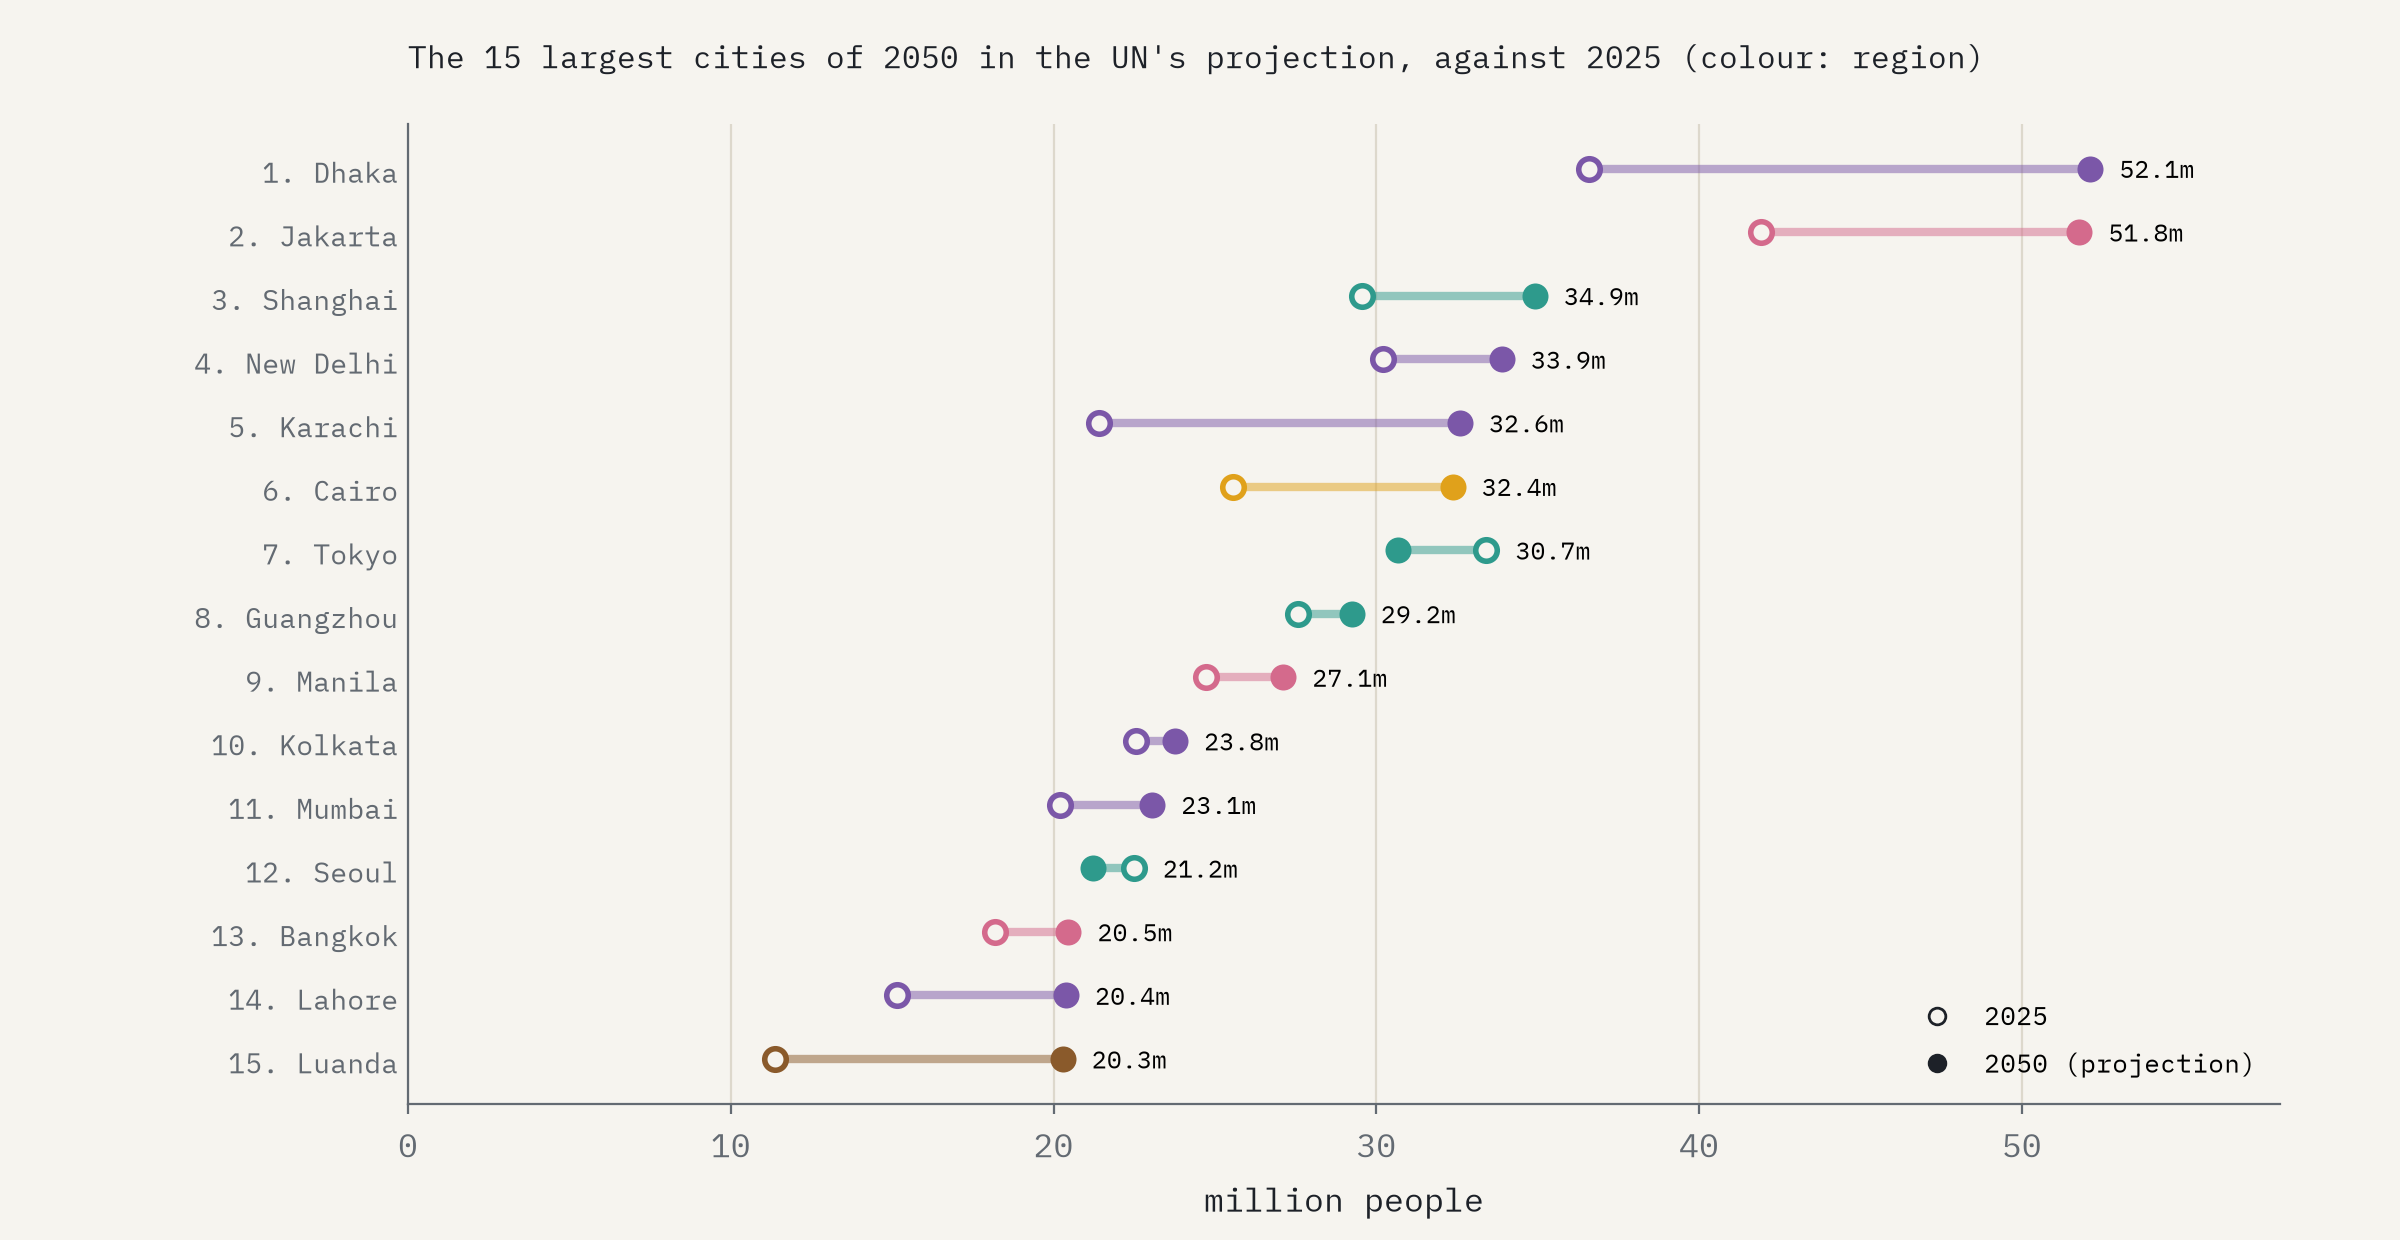
\includegraphics[width=\textwidth]{f_2050.png}
\caption{The 15 largest cities of 2050 in the UN's projection, 2025 (open) and 2050 (solid).}\label{fig:2050}\end{figure}

\section{Limitations}
First, the historical figures are estimates, often rounded and inferred from walls, house counts, supplies or later censuses; a factor of two is plausible for ancient cities, and the compilations disagree. Second, coverage is uneven: before AD 1000 the compilations hold 11 places in the Americas and 4 in sub-Saharan Africa, against hundreds in Europe and Asia later (Table~\ref{tab:cov}); absence is not evidence of absence. Third, Modelski's thresholds create ties and hide places below 100,000 after 1000 BC. Fourth, interpolation and averaging are choices; at the historical snapshots 14.7\% of top-ten estimates involve interpolation. Fifth, the 1975 seam joins agglomeration-style historical figures to DEGURBA cities; I report it rather than adjust it. Sixth, 2030 to 2050 are projections. Seventh, the certainty score of \citet{reba} concerns identification and placement, not the population figure.

\begin{table}[tbp]\centering\footnotesize\setlength{\tabcolsep}{4pt}\caption{Places with at least one estimate, by region and period (Chandler and Modelski, after corrections).}\label{tab:cov}\begin{tabular}{lrrrrr}\toprule Region & Before 1000 BC & 1000 BC to AD 999 & 1000 to 1499 & 1500 to 1799 & 1800 to 1975\\\midrule
West and Central Asia & 46 & 60 & 52 & 39 & 93\\
North Africa & 8 & 14 & 19 & 17 & 28\\
Europe & 6 & 56 & 177 & 241 & 592\\
South Asia & 4 & 31 & 46 & 78 & 189\\
East Asia & 5 & 41 & 48 & 67 & 174\\
South-East Asia and Oceania & 0 & 5 & 15 & 19 & 59\\
Sub-Saharan Africa & 0 & 4 & 13 & 29 & 67\\
North America & 0 & 0 & 4 & 6 & 132\\
Latin America and the Caribbean & 0 & 11 & 12 & 47 & 93\\
\bottomrule\end{tabular}\end{table}

\section{Conclusion}
For most of six thousand years the largest city lay in a belt from Egypt and Mesopotamia to China. The industrial nineteenth century pulled the centre of the urban world to the North Atlantic for about a century; it has since returned to Asia, further south than ever before. The sources disagree often enough that any single list should be read as one defensible reading of uncertain evidence, which is how this one is offered.

\section*{Data and code availability}
The interactive map is at \url{https://maps.tristanhotham.com/largest-cities/}. Data and code are at \url{https://github.com/Tristan-Hotham/largest-cities} and archived with this paper at https://doi.org/10.5281/zenodo.23872999. Derived data and text are released under CC BY 4.0 and code under the MIT licence. Historical data: Reba, Reitsma and Seto (2016), CC BY 4.0. UN data: World Urbanization Prospects 2025, CC BY 3.0 IGO.

\section*{AI statement}
I wrote the text, with drafting and editing assistance from Claude (Anthropic), which also helped prepare the analysis code. I reviewed and checked all text and results.

\begin{thebibliography}{9}
\bibitem[Chandler(1987)]{chandler} Chandler, T. (1987) \textit{Four Thousand Years of Urban Growth: An Historical Census}. Lewiston: St David's University Press.
\bibitem[Modelski(2003)]{modelski} Modelski, G. (2003) \textit{World Cities: -3000 to 2000}. Washington: FAROS 2000.
\bibitem[Reba et al.(2016)]{reba} Reba, M., Reitsma, F. and Seto, K. C. (2016) Spatializing 6,000 years of global urbanization from 3700 BC to AD 2000. \textit{Scientific Data} 3, 160034. \url{https://doi.org/10.1038/sdata.2016.34}
\bibitem[Reba(2016a)]{figc} Reba, M. (2016) Chandler Population Data. figshare, CC BY 4.0. \url{https://doi.org/10.6084/m9.figshare.2059494.v3}
\bibitem[Reba(2016b)]{figa} Reba, M. (2016) Modelski Ancient Period Data. figshare, CC BY 4.0. \url{https://doi.org/10.6084/m9.figshare.2059497.v2}
\bibitem[Reba(2016c)]{figm} Reba, M. (2016) Modelski Modern Period Data. figshare, CC BY 4.0. \url{https://doi.org/10.6084/m9.figshare.2059500.v3}
\bibitem[United Nations(2025)]{wup} United Nations, Department of Economic and Social Affairs, Population Division (2025) World Urbanization Prospects: The 2025 Revision, files 18 to 21. CC BY 3.0 IGO.
\bibitem[Natural Earth(2026)]{ne} Natural Earth (2026) Admin 0 countries and land, 1:50m. Public domain. \url{https://www.naturalearthdata.com/}
\end{thebibliography}
\end{document}
